\documentclass[11pt]{article}

\usepackage{amsmath, amsthm, amssymb}
\usepackage{enumerate}
\usepackage{pdflscape}
\usepackage{caption}
\usepackage{bm}

\usepackage{ifpdf}
\ifpdf
\usepackage[pdftex]{graphicx}
\else
\usepackage[dvips]{graphicx}
\fi
\usepackage{tikz}
 	 \usetikzlibrary{arrows,backgrounds}
\usepackage[all]{xy}

\usepackage{multicol}

\usepackage{tocvsec2}

\usepackage{bbm}

\input xy
\xyoption{all}

\usepackage[pdftex,plainpages=false,hypertexnames=false,pdfpagelabels]{hyperref}
\newcommand{\arxiv}[1]{\href{http://arxiv.org/abs/#1}{\tt arXiv:\nolinkurl{#1}}}
\newcommand{\arXiv}[1]{\href{http://arxiv.org/abs/#1}{\tt arXiv:\nolinkurl{#1}}}
\newcommand{\doi}[1]{\href{http://dx.doi.org/#1}{{\tt DOI:#1}}}
\newcommand{\euclid}[1]{\href{http://projecteuclid.org/getRecord?id=#1}{{\tt #1}}}
\newcommand{\mathscinet}[1]{\href{http://www.ams.org/mathscinet-getitem?mr=#1}{\tt #1}}
\newcommand{\googlebooks}[1]{(preview at \href{http://books.google.com/books?id=#1}{google books})}
\newcommand{\Ws}{\text{W*}}

\usepackage{xcolor}
\definecolor{dark-red}{rgb}{0.7,0.25,0.25}
\definecolor{dark-blue}{rgb}{0.15,0.15,0.55}
\definecolor{medium-blue}{rgb}{0,0,.8}
\definecolor{shaded-blue}{RGB}{98,140,255}
\definecolor{DarkGreen}{RGB}{0,150,0}
\definecolor{rho}{named}{red}
\definecolor{Salmon}{RGB}{255, 144, 144}
\hypersetup{
   colorlinks, linkcolor={purple},
   citecolor={medium-blue}, urlcolor={medium-blue}
}

%\addtolength{\textwidth}{.5in}
\usepackage{longtable}
\usepackage{fullpage}
%\renewcommand{\arraystretch}{1.5}

% Page size %%%%%%%%%%%%%%%%%%%%%%%%%%%%%%%%%%%%%%%%%%%
\setlength\topmargin{-.25in}
\setlength\headheight{0in}
\setlength\headsep{.2in}
\setlength\textheight{9in}
%\addtolength{\hoffset}{-0.25in}
%\addtolength{\textwidth}{.5in}
\setlength\parindent{0.25in}

% Theorems %%%%%%%%%%%%%%%%%%%%%%%%%%%%%%%%%%%%%%%%%%
\theoremstyle{plain}
\newtheorem{thm}{Theorem}[section]
\newtheorem*{thm*}{Theorem}
\newtheorem{thmalpha}{Theorem}
\renewcommand*{\thethmalpha}{\Alph{thmalpha}}
\newtheorem{cor}[thm]{Corollary}
\newtheorem{coralpha}[thmalpha]{Corollary}
\newtheorem*{cor*}{Corollary}
\newtheorem{conj}[thm]{Conjecture}
\newtheorem{conjalpha}[thmalpha]{Conjecture}
\newtheorem*{conj*}{Conjecture}
\newtheorem{lem}[thm]{Lemma}
\newtheorem{fact}[thm]{Fact}
\newtheorem{facts}[thm]{Facts}
\newtheorem{prop}[thm]{Proposition}
\newtheorem{quest}[thm]{Question}
\newtheorem*{quest*}{Question}
\newtheorem*{claim*}{Claim}
\newtheorem{quests}[thm]{Questions}
\theoremstyle{definition}
\newtheorem{defn}[thm]{Definition}
\newtheorem{construction}[thm]{Construction}
\newtheorem{alg}[thm]{Algorithm}
\newtheorem{assumption}[thm]{Assumption}

\newtheorem{nota}[thm]{Notation}
\newtheorem{nb}[thm]{Note}
\newtheorem{note}[thm]{Note}
\newtheorem{exs}[thm]{Examples}
\newtheorem{ex}[thm]{Example}
\newtheorem{exercise}[thm]{Exercise}
\newtheorem{sub-ex}[thm]{Sub-Example}
\newtheorem{rem}[thm]{Remark}
\newtheorem*{rem*}{Remark}
\newtheorem{remark}[thm]{Remark}
\newtheorem{rems}[thm]{Remarks}
\newtheorem{warn}[thm]{Warning}

% Figure Numbering %%%%%%%%%%%%%%%%%%%%%%%%%%%%%%%%%%%
%\usepackage{chngcntr} %Numbers figures by section
%\counterwithin{figure}{section}

% Operators %%%%%%%%%%%%%%%%%%%%%%%%%%%%%%%%%%%%%%%%%%%
\DeclareMathOperator{\Ad}{Ad}
\DeclareMathOperator{\Aut}{Aut}
\DeclareMathOperator{\coev}{coev}
\DeclareMathOperator{\Dom}{Dom}
\DeclareMathOperator{\End}{End}
\DeclareMathOperator{\ev}{ev}
\DeclareMathOperator{\Hom}{Hom}
\DeclareMathOperator{\Mor}{Mor}
\DeclareMathOperator{\op}{op}
\DeclareMathOperator{\ONB}{ONB}
\DeclareMathOperator{\Ob}{Ob}
\DeclareMathOperator{\rev}{rev}
\DeclareMathOperator{\spann}{span}
\DeclareMathOperator{\supp}{supp}
\DeclareMathOperator{\id}{id}
\DeclareMathOperator{\Isom}{Isom}
\DeclareMathOperator{\ind}{ind}
\DeclareMathOperator{\im}{im}
\DeclareMathOperator{\Irr}{Irr}
\DeclareMathOperator{\Spec}{Spec}
\DeclareMathOperator{\Stab}{Stab}
\DeclareMathOperator{\Tr}{Tr}
\DeclareMathOperator{\tr}{tr}
\DeclareMathOperator{\Gr}{Gr}


% Math %%%%%%%%%%%%%%%%%%%%%%%%%%%%%%%%%%%%%%%%%%%%%
\newcommand{\D}{\displaystyle}
\newcommand{\comment}[1]{}
\newcommand{\hs}{\hspace{.07in}}
\newcommand{\hsp}[1]{\hs\text{#1}\hs}
\newcommand{\be}{\begin{enumerate}[label=(\arabic*)]}
\newcommand{\ee}{\end{enumerate}}
\newcommand{\itm}[1]{\item[\underline{\ensuremath{#1}:}]}
\newcommand{\itt}[1]{\item[\underline{\text{#1}:}]}
\newcommand{\N}{\mathbb{N}}
\newcommand{\Natural}{\mathbb{N}}
\newcommand{\Z}{\mathbb{Z}}
\newcommand{\Q}{\mathbb{Q}}
\newcommand{\F}{\mathbb{F}}
\newcommand{\R}{\mathbb{R}}
\newcommand{\C}{\mathbb{C}}
\newcommand{\B}{\mathbb{B}}
\renewcommand{\P}{\mathbb{P}}
\newcommand{\I}{\infty}
\newcommand{\set}[2]{\left\{#1 \middle| #2\right\}}
\newcommand{\thh}{^{\text{th}}}
\renewcommand{\a}{\mathfrak{a}}
\renewcommand{\b}{\mathfrak{b}}
\renewcommand{\c}{\mathfrak{c}}
\newcommand{\n}{\mathfrak{n}}
\newcommand{\m}{\mathfrak{m}}
\newcommand{\bbOne}{\mathbbm{1}}
\renewcommand{\alg}[1]{{\bm{\langle} #1\bm{\rangle}}}


% some math commands specific to this document %%%%%%%%%%%%
\newcommand{\xalt}{x^{\text{alt}\otimes n}}
\newcommand{\xbaralt}{\overline{x}^{\text{alt}\otimes n}}
\newcommand{\act}{\overline{x}^{?}}
%%%%%%%%%%%%%%%%%%%%%%%%%%%%

\newcommand{\dave}[1]{\marginpar{\tiny \textcolor{orange}{DP: #1}}}
\newcommand{\corey}[1]{\marginpar{\tiny \textcolor{green}{CJ: #1}}}
\newcommand{\Af}{\mathcal{A}\Lambda_{F}}
\newcommand{\WStar}{\bfW\text{*}}
%\newcommand{\Irr}{\text{Irr}(\mathcal{C})}

% tricky way to iterate macros over a list
\def\semicolon{;}
\def\applytolist#1{
    \expandafter\def\csname multi#1\endcsname##1{
        \def\multiack{##1}\ifx\multiack\semicolon
            \def\next{\relax}
        \else
            \csname #1\endcsname{##1}
            \def\next{\csname multi#1\endcsname}
        \fi
        \next}
    \csname multi#1\endcsname}

% \def\cA{{\cal A}} for A..Z
\def\calc#1{\expandafter\def\csname c#1\endcsname{{\mathcal #1}}}
\applytolist{calc}QWERTYUIOPLKJHGFDSAZXCVBNM;
% \def\bbA{{\mathbb A}} for A..Z
\def\bbc#1{\expandafter\def\csname bb#1\endcsname{{\mathbb #1}}}
\applytolist{bbc}QWERTYUIOPLKJHGFDSAZXCVBNM;
% \def\bfA{{\mathbf A}} for A..Z
\def\bfc#1{\expandafter\def\csname bf#1\endcsname{{\mathbf #1}}}
\applytolist{bfc}QWERTYUIOPLKJHGFDSAZXCVBNM;
% \def\sA{{\sf A}} for A..Z
\def\sfc#1{\expandafter\def\csname s#1\endcsname{{\sf #1}}}
\applytolist{sfc}QWERTYUIOPLKJHGFDSAZXCVBNM;
% \def\fA{{\mathfrak A}} for A..Z
\def\fc#1{\expandafter\def\csname f#1\endcsname{{\mathfrak #1}}}
\applytolist{fc}QWERTYUIOPLKJHGFDSAZXCVBNM;


\newcommand{\PA}{\cP\hspace{-.1cm}\cA}
\newcommand{\Fun}{{\sf Fun}}
\newcommand{\Rep}{{\sf Rep}}
\newcommand{\Set}{{\sf Set}}
\newcommand{\FreeMod}{{\sf FreeMod}}
\newcommand{\Mod}{{\sf Mod}}
\newcommand{\Proj}{{\sf Proj}}
\newcommand{\AlgBim}{{\sf AlgBim}}
\newcommand{\Bim}{{\sf Bim}}
\newcommand{\bfBim}{{\sf Bim_{bf}}}
\newcommand{\spBim}{{\sf Bim^{sp}}}
\newcommand{\spbfBim}{{\sf Bim_{bf}^{sp}}}
\renewcommand{\Vec}{{\sf Vec}}
\newcommand{\fdVec}{{\sf Vec_{fd}}}
\newcommand{\Hilb}{{\sf Hilb}}
\newcommand{\fdHilb}{{\sf Hilb_{fd}}}
\newcommand{\ConAlg}{{\sf ConAlg}}
\newcommand{\DisInc}{{\sf DisInc}}


\newcommand{\jw}[1]{f^{(#1)}}
\newcommand{\todo}[1]{\textcolor{blue}{\textbf{TODO: #1}}}
\newcommand{\nn}[1]{\textcolor{red}{[[#1]]}}
\newcommand{\noshow}[1]{}
\newcommand{\MR}[1]{}
\newcommand{\TL}{\cT\hspace{-.08cm}\cL}
\newcommand{\rhoE}{\textcolor{rho}{e_1}}
\newcommand{\rhoJW}{\textcolor{rho}{\jw{2}}}


% TikZ operators %%%%%%%%%%%%%%%%%%%%%%%%%%%%%%%%%%%%%%%%
\usetikzlibrary{shapes}
\usetikzlibrary{cd}
\usetikzlibrary{backgrounds}
\usetikzlibrary{decorations,decorations.pathreplacing,decorations.markings}
\usetikzlibrary{fit,calc,through}
\usetikzlibrary{external}
\usetikzlibrary{arrows}
\tikzset{vertex/.style = {shape=circle,draw,fill=black,inner sep=0pt,minimum size=5pt}}
\tikzset{edge/.style = {->,> = latex', bend right}}
\tikzset{
	super thick/.style={line width=3pt}
}
\tikzset{
    quadruple/.style args={[#1] in [#2] in [#3] in [#4]}{
        #1,preaction={preaction={preaction={draw,#4},draw,#3}, draw,#2}
    }
}
\tikzstyle{shaded}=[fill=gray!25!white]
\tikzstyle{shadedpink}=[left color= white, right color = Salmon]
\tikzstyle{unshaded}=[fill=white]
\tikzstyle{empty box}=[circle, draw, thick, fill=white, opaque, inner sep=2mm]
\tikzstyle{annular}=[scale=.7, inner sep=1mm, baseline]
\tikzstyle{rectangular}=[scale=.75, inner sep=1mm, baseline=-.1cm]
\tikzstyle{mid>}=[decoration={markings, mark=at position 0.5 with {\arrow{>}}}, postaction={decorate}]
\tikzstyle{mid<}=[decoration={markings, mark=at position 0.5 with {\arrow{<}}}, postaction={decorate}]
\tikzstyle{over}=[double, draw=white, super thick, double=]
\tikzstyle{relativecommutantshading}=[fill=blue!20!white]
\tikzstyle{ctwoshading}=[fill=red!15!white]

\newcommand{\roundNbox}[6]{
	\draw[rounded corners=5pt, very thick, #1] ($#2+(-#3,-#3)+(-#4,0)$) rectangle ($#2+(#3,#3)+(#5,0)$);
	\coordinate (ZZa) at ($#2+(-#4,0)$);
	\coordinate (ZZb) at ($#2+(#5,0)$);
	\node at ($1/2*(ZZa)+1/2*(ZZb)$) {#6};
}


\newcommand{\nbox}[6]{
	\draw[thick, #1] ($#2+(-#3,-#3)+(-#4,0)$) rectangle ($#2+(#3,#3)+(#5,0)$);
	\coordinate (ZZa) at ($#2+(-#4,0)$);
	\coordinate (ZZb) at ($#2+(#5,0)$);
	\node at ($1/2*(ZZa)+1/2*(ZZb)$) {#6};
}

\newcommand{\ncircle}[4]{
	\draw[very thick, #1] #2 circle (#3);
	\node at #2 {#4};
%	\filldraw[red] ($#2+(#4:#3cm)$) circle (.05cm);
%	\node at ($#2+(#4:.15cm)+(#4:#3cm)$) {$\star$};
}

  \newcommand{\tikzmath}[2][]
     {\vcenter{\hbox{\begin{tikzpicture}[#1]#2
                     \end{tikzpicture}}}
     }

% premade TIKZ stuff %%%%%%%%%%%%%%%%%%%%%%%%%%%%
\newcommand{\uscircle}{
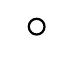
\begin{tikzpicture}
\draw[thick] (0,0) circle (1mm) ;
\end{tikzpicture}
}

\newcommand{\scircle}{

\begin{tikzpicture}
\filldraw[thick][shaded] (0,0) circle (1mm);
\end{tikzpicture}
}

% colors %%%%%%%%%%%%%%%%%%%%%%%%%%%%%%%%%%%%%%%%
\newcommand{\cupcolor}{DarkGreen}
\newcommand{\alphacolor}{blue}
\newcommand{\betacolor}{red}

% title %%%%%%%%%%%%%%%%%%%%%%%%%%%%%%%%%%%%%%%%%

\title{Module embedding via towers of algebras}
\author{Desmond Coles, Peter Huston, David Penneys, \& Srivatsa Srinivas}





%%%%%%%%%%%%%%%%%%%%%%%%%%%%%%%%%%%%%%


\usepackage[utf8]{inputenc}
\begin{document}


%%%%%%%%%%%%%%%%%%%%%%%%%%%%%%%%%%%%%%%%%%%%%%%%%%%%%%%%%%%%%%%
%%%%%%%%%%%%%%%%%%%%%%%%%%%%%%%%%%%%%%%%%%%%%%%%%%%%%%%%%%%%%%%
%%%%%%%%%%%%%%%%%%%%%%%%%%%%%%%%%%%%%%%%%%%%%%%%%%

\maketitle
\begin{abstract}
Jones and Penneys have shown that a finite depth subfactor planar $*$-algebra embeds in the bipartite graph planar algebra of its principal graph. By constructing a strongly Markov inclusion of finite von Neumann algebras from a given module, we extend their techniques to the case of cyclic modules over a subfactor planar algebra, relating the calculus of string diagrams in a module category and the canonical planar $*$-algebra structure on a Markov inclusion. We generalize their result, showing that a finite depth subfactor $*$-planar algebra embeds into the bipartite graph planar algebra of the fusion graph of any of its cyclic modules. 
\end{abstract}
\section{Introduction}



%%%%%%%%%%%%%%%%%%%%%%%%%%%%%%%%%%%%%%%%%%%%%%%%%%%%%%%
%%%%%%%%%%%%%%%%%%%%%%%%%%%%%%%%%%%%%%%%%%%%%%%%%%%%%%%
%%%%%%%%%%%%%%%%%%%%%%%%%%%%%%%%%%%%%%%%%%%%%%%%%%%%%%%
\section{The canonical planar algebra of a strongly Markov inclusion} 
\label{sec:StronglyMarkovPA}



%%%%%%%%%%%%%%%%%%%%%%%%%%%%%%%%%%%%%%%%%%%%%%%%%%%%%%%
\subsection{Strongly Markov inclusions} 

\nn{define stronlgy Markov inclusion of finite von Neumann algebras}

Recall that if $M_0\subseteq (M_1,\tr_1)$ is a strongly Markov inclusion of finite dimensional von Neumann algebras with $[M_1:M_0]=d^2$ then we can iterate the basic construction to obtain a tower of algebras and there is a canonical planar algebra strucutre on this tower, called the \textit{canonical planar $\ast$-algebra of a strongly Markov inclusion} corresponding to $M_0\subseteq (M_1,\tr_1)$. One important feature of this construction is that it depends on the existence of a Pimsner-Popa basis for $M_1$ over $M_0$. 
We refer the reader to \cite{MR2812459} for more details on this construction. 
We will need the following:

\begin{prop}[{\cite[Prop 2.25]{penneys}}]\label{iso}
For any $n$, the map:
\[
\theta_n: \bigotimes_{M_0}^{n}M_1 \rightarrow M_n
\]
defined by $x_1\otimes\cdots x_n \mapsto x_1v_1x_2v_2\cdots x_nv_n$, where $v_k:=d^ne_ne_{n-1}\cdots e_1$, is an $M_1-M_1$ bimodule isomorphism.
\end{prop}

For the following definition, we will always assume shaded planar tangles are in \textit{standard form}, meaning:
\begin{itemize}
\item All input/output disks are parallel rectangles.
\item All strings are smooth, strings emanating from the input disks come from the top of the disk, and strings connected to the output disk connect to the top.
\item The maxima and minima of any two strings occurs at different heights, and no extrema ever occurs at the same height as that of the top or bottom of a rectangle.
\item The $\ast$ of a tangle is always on the left edge of the boundary rectangle.

\end{itemize}

%%%%%%%%%%%%%%%%%%%%%%%%%%%%%%%%%%%%%%%%%%%%%%%%%%%%%%%
\subsection{Defining the planar algebra} 


\begin{defn} 
The canonical planar $\ast$-algebra of a strongly Markov inclusion $M_0\subseteq (M_1,\tr_1)$ is defined as follows:

	The box spaces are $P_{n,+}:=\theta_n^{-1}(M_0'\cap M_{n}) $ and $P_{n,-}:=\theta_n^{-1}(M_1'\cap M_{n+1})$. Suppose a tangle $T$ has type $(r,\pm)$ and $s$ input rectangles of types $(r_i,\pm_i)$. If we arrange $T$ in standard form, the action of $T$ can be understood by reading the tangle from top to bottom, moving a horizontal line upwards. At the bottom, we begin with $1\in M_i$, where $i$ is $0$ if $T$ has type $(r,+)$ and $1$ if $T$ has type $(r,-)$. By the top, we will have produced an element of $M_i$-invariant element of $M_{r+i}$, depending on a choice of pure tensor $\nu=\otimes_{i=1}^r\nu_i\in\otimes_{i=1}^rP_{r_i,\pm_i}$. Let $n_y$ be the number of shaded regions intersected by a horizontal line at a height $y$. We first consider $y$ such that the horizontal line intersects no input disks or extrema of strands. At these levels, one can read off an $M_i$-invariant element $\eta_y\in \otimes^{n_y}M_1$, which remains constant as long as the horizontal line intersects no disks or extrema. One should think of shaded regions as representing elements of $M_1$ and the unshaded regions as representing $\otimes_{M_0}$. We will now describe what happens when the line moves upwards and passes through extrema of the strings and input rectangles:
	\begin{itemize}
	\item If the horizontal line passes through the $j$-th input rectangle and there are $t$ shaded regions to the left of it, and it has type $(r_j,+)$, then at vertical height $y$, we insert $\nu_j$ into $\eta_y$ in the following way:
	\[
	x_1\otimes\cdots x_{n_y} \mapsto x_1\otimes \cdots x_t\otimes \nu_j \otimes x_{t+1}\otimes \cdots x_{n_y}
	\]
	 If the rectangle has type $(r_j,+)$, then at vertical height $y$, we insert $\nu_j$ into	$\eta_y$ in the following way:
	\[
	x_1\otimes\cdots x_{n_y} \mapsto x_1\otimes \cdots x_t \nu_j \otimes x_{t+1}\otimes \cdots x_{n_y}=x_1\otimes \cdots \nu_j x_t  \otimes x_{t+1}\otimes \cdots x_{n_y}
	\]
	Both of these maps are well-defined, by \cite[Lem2.29]{penneys}.
	\item The effect of passing upwards through the extrema of a strand is as follows: 
\begin{align*}
	&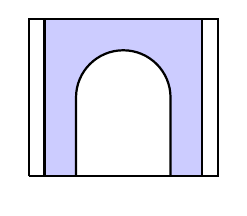
\begin{tikzpicture}[baseline]
		\fill[unshaded](-1.2,-1) -- (-1.2,1) -- (-1,1) -- (-1,-1) -- (-1.2,-1);
		\fill[unshaded](1.2,-1) -- (1.2,1) -- (1,1) -- (1,-1) -- (1.2,-1);
		\fill[relativecommutantshading] (-1,-1) -- (-1,1) -- (1,1) -- (1,-1) -- (-1,-1);
		\fill[unshaded] (.6,-1) -- (.6,0) arc (0:180:.6cm) -- (-.6,-1);
		\draw[thick] (.6,-1) -- (.6,0) arc (0:180:.6cm) -- (-.6,-1);
		\draw[thick] (-1,-1) -- (-1,1) -- (1,1) -- (1,-1) -- (-1,-1);
		\draw[thick] (-1.2,-1) -- (-1.2,1) -- (1.2,1) -- (1.2,-1) -- (-1.2,-1);
	\end{tikzpicture}
	: x\otimes y\mapsto xy \\
	&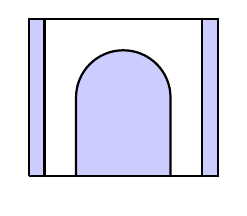
\begin{tikzpicture}[baseline]
		\fill[relativecommutantshading](-1.2,-1) -- (-1.2,1) -- (-1,1) -- (-1,-1) -- (-1.2,-1);
		\fill[relativecommutantshading](1.2,-1) -- (1.2,1) -- (1,1) -- (1,-1) -- (1.2,-1);
		\fill[unshaded] (-1,-1) -- (-1,1) -- (1,1) -- (1,-1) -- (-1,-1);
		\fill[relativecommutantshading] (.6,-1) -- (.6,0) arc (0:180:.6cm) -- (-.6,-1);
		\draw[thick] (.6,-1) -- (.6,0) arc (0:180:.6cm) -- (-.6,-1);
		\draw[thick](-1,-1) -- (-1,1) -- (1,1) -- (1,-1) -- (-1,-1);
		\draw[thick] (-1.2,-1) -- (-1.2,1) -- (1.2,1) -- (1.2,-1) -- (-1.2,-1);
	\end{tikzpicture}
	: x\otimes y \otimes z \mapsto dxE_{M_0}(y)\otimes z=dx\otimes E_{M_0}(y) z \\
	&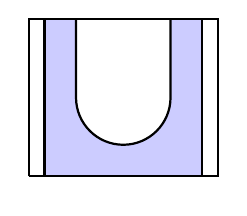
\begin{tikzpicture}[baseline]
		\fill[unshaded](-1.2,-1) -- (-1.2,1) -- (-1,1) -- (-1,-1) -- (-1.2,-1);
		\fill[unshaded](1.2,-1) -- (1.2,1) -- (1,1) -- (1,-1) -- (1.2,-1);
		\fill[relativecommutantshading] (-1,-1) -- (-1,1) -- (1,1) -- (1,-1) -- (-1,-1);
		\fill[unshaded] (.6,1) -- (.6,0) arc (0:-180:.6cm) -- (-.6,1);
		\draw[thick] (.6,1) -- (.6,0) arc (0:-180:.6cm) -- (-.6,1);
		\draw[thick](-1,-1) -- (-1,1) -- (1,1) -- (1,-1) -- (-1,-1);
		\draw[thick] (-1.2,-1) -- (-1.2,1) -- (1.2,1) -- (1.2,-1) -- (-1.2,-1);
	\end{tikzpicture}
	: x \mapsto d^{-1}\sum\limits_{b\in B}xb\otimes b^{\ast}=d^{-1}\sum\limits_{b\in B}b\otimes b^{\ast} x \\
	&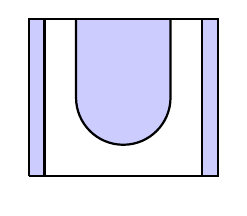
\begin{tikzpicture}[baseline]
		\fill[relativecommutantshading](-1.2,-1) -- (-1.2,1) -- (-1,1) -- (-1,-1) -- (-1.2,-1);
		\fill[relativecommutantshading](1.2,-1) -- (1.2,1) -- (1,1) -- (1,-1) -- (1.2,-1);
		\fill[unshaded] (-1,-1) -- (-1,1) -- (1,1) -- (1,-1) -- (-1,-1);
		\fill[relativecommutantshading] (.6,1) -- (.6,0) arc (0:-180:.6cm) -- (-.6,1);
		\draw[thick] (.6,1) -- (.6,0) arc (0:-180:.6cm) -- (-.6,1);
		\draw[thick](-1,-1) -- (-1,1) -- (1,1) -- (1,-1) -- (-1,-1);
		\draw[thick] (-1.2,-1) -- (-1.2,1) -- (1.2,1) -- (1.2,-1) -- (-1.2,-1);
	\end{tikzpicture}
	: x\otimes y \mapsto x\otimes 1 \otimes y 
\end{align*}
	
\end{itemize} 
The $\ast$-structure of the planar algebra is described in \cite{planaralg1}.
\end{defn}

%We will proceed with the same general technique for defining the embedding of planar algebras as in \cite{penneys}, in that we will also initially embed into the canonical $\ast$-planar algebra, and then make use of the following theorem:

%\begin{thm}[Penneys, Jones, \cite{penneys}] \label{planaralgebraisomorphism}
%The canonical planar $\ast$-algebra associated the strongly Markov inclusion $M_0\subseteq (M_1,\tr_1)$ is isomorphic to the bipartite graph planar $\ast$-algebra of the Bratteli diagram for the inclusion $M_0\subseteq M_1$.
%\end{thm}

%%%%%%%%%%%%%%%%%%%%%%%%%%%%%%%%%%%%%%%%%%%%%%%%%%%%%%%
\subsection{The shift isomorphism} 

In this article, we will make extensive use of the following lemma adapted from \cite[Lem.~2.49]{MR2812459}, which provides sufficient conditions for a collection of maps to be a morphism of shaded planar $\dag$-algebras.

\begin{lem}[{\cite[Variation of Lem.~2.49]{MR2812459}}]
\label{lem:SufficientConditionsForPlanarMap}
Suppose $\Phi_{n,\pm} : \cP_{n,\pm} \to \cQ_{n,\pm}$ is a collection of unital $\dag$-algebra maps such that
\begin{enumerate}[(1)]
\item
$\Phi$ maps Jones projections in $\cP_{n,+}$ to Jones projections in $\cQ_{n,+}$,
\item
$\Phi$ commutes with the action of the following tangles:
$$
\underset{
\substack{
\text{right inclusion}
\\ 
\cP_{n,+} \to \cP_{n+1,+}
}}
{
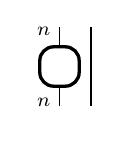
\begin{tikzpicture}
	\draw (.4,-.5) -- (.4,.5);
	\draw (0,-.5) -- (0,.5);
	\node at (-.2,.45) {\scriptsize{$n$}};
	\node at (-.2,-.45) {\scriptsize{$n$}};
	\roundNbox{unshaded}{(0,0)}{.25}{0}{0}{}
\end{tikzpicture}
}
\qquad\qquad
\underset{
\substack{
\text{left inclusion}
\\ 
\cP_{n,-} \to \cP_{n+1,+}
}}
{
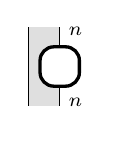
\begin{tikzpicture}[xscale=-1]
	\fill[shaded] (.4,-.5) -- (.4,.5) -- (0,.5) -- (0,-.5);
	\draw (.4,-.5) -- (.4,.5);
	\draw (0,-.5) -- (0,.5);
	\node at (-.2,.45) {\scriptsize{$n$}};
	\node at (-.2,-.45) {\scriptsize{$n$}};
	\roundNbox{unshaded}{(0,0)}{.25}{0}{0}{}
\end{tikzpicture}
}
\qquad\qquad
\underset{
\substack{
\text{right capping}
\\ 
\cP_{n,+} \to \cP_{n-1,+}
}}
{
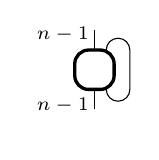
\begin{tikzpicture}
	\draw (.15,-.25) arc (-180:0:.15cm) -- (.45,.25) arc (0:180:.15cm);
	\draw (0,-.5) -- (0,.5);
	\node at (-.4,.45) {\scriptsize{$n-1$}};
	\node at (-.4,-.45) {\scriptsize{$n-1$}};
	\roundNbox{unshaded}{(0,0)}{.25}{0}{0}{}
\end{tikzpicture}
}
\qquad\qquad
\underset{
\substack{
\text{left capping}
\\ 
\cP_{n,+} \to \cP_{n-1,-}
}}
{
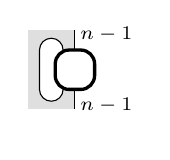
\begin{tikzpicture}[xscale=-1]
	\fill[shaded] (.6,-.5) -- (.6,.5) -- (0,.5) -- (0,-.5);
	\filldraw[unshaded] (.15,-.25) arc (-180:0:.15cm) -- (.45,.25) arc (0:180:.15cm);
	\draw (0,-.5) -- (0,.5);
	\node at (-.4,.45) {\scriptsize{$n-1$}};
	\node at (-.4,-.45) {\scriptsize{$n-1$}};
	\roundNbox{unshaded}{(0,0)}{.25}{0}{0}{}
\end{tikzpicture}
}.
$$
\end{enumerate}
Then $\Phi$ is a morphism of shaded planar $\dag$-algebras.
\end{lem}

\nn{TODO: the canonical planar algebra for $A_0 \subset A_1$ is canonically iso to the canonical planar algebra for $A_2\subset A_3$ when $A_0\subset A_1$ is a strongly Markov inclusion.}


%%%%%%%%%%%%%%%%%%%%%%%%%%%%%%%%%%%%%%%%%%%%%%%%%%%%%%%
\subsection{The compression isomorphism} 

The following lemma is well known to experts. 
We provide a proof for convenience and completeness.

\begin{lem}
Suppose $N\subset M\subset B(H)$ is an inclusion of von Neumann algebras and $p\in P(N)$.
\begin{enumerate}[(1)]
\item
$p(N'\cap M) = pN' \cap pMp$.
\item
Suppose the central support of $p$ in $N$ is $z\in Z(N)$.
The map $x\mapsto px$ is an isomorphism $z(N'\cap M) \to p(N'\cap M)$.
\end{enumerate}
\end{lem}
\begin{proof}
\mbox{}
\item[\underline{Proof of (1):}]
The proof of (1) is similar to the proof of the standard fact that $(pNp)' = N'p$.

Clearly $(N'\cap M)p \subseteq (N'p) \cap pMp$.
Suppose $u$ is a unitary in $(N'p) \cap pMp$.
Let $K$ be the closure of $NpH$.
Let $q\in B(H)$ be the projection onto $K$, which is clearly in $N' \cap N = Z(N)$.
Define $u_0$ in $B(K)$ by $u_0 (np\xi) := npu\xi$.
One now verifies that $u_0$ is an isometry and thus is well-defined.
Look at the operator $u_0q \in N' \cap B(H)$, and note that $u = u_0qp \in N'p$.
We claim that $u_0q \in M$, so that $u = u_0qp \in (N' \cap M)p$.
First, for any $m \in M'$, $n \in N$, and $\xi\in H$,
we have
$mu_0np\xi  = mnup\xi = nupm\xi = u_0npm\xi = u_0mnp\xi$.
Thus $u_0 \in qMq$.
Since $q \in M$, for all $m \in M'$, we have $u_0qm\xi = u_0mq\xi = mu_0q\xi$.
Hence $u_0q$ commutes with $M'$ on $H$, and $u_0q \in M$. 

\item[\underline{Proof of (2):}]
For $x\in N'\cap M$, we have $p(zx) = px$.
Hence the map is surjective.
We now show the map is injective.
Suppose $x \in z(N'\cap M)$ such that $px = 0$.
By (1), $z(N'\cap M) = zN' \cap zMz$.
Then for all unitaries $u\in U(N)$, $upz = z(up) \in zN$, so 
$0 = upxu^* = (upz)xu^* = x(upzu^*) = xupu^*$.
Taking sup over $u \in U(N)$ yields $0 = xz = x$.
\end{proof}

\nn{edit below here -- math taken from elsewhere, OK to use.}




\begin{thm}
\label{thm:IsomorphicStandardInvariants}
Suppose $M_0\subset M_1$ is a strongly Markov inclusion of finite von Neumann algebras and $p\in M_0$ is a nonzero projection with central support $1$.
Then 
\begin{enumerate}
\item
The inclusion $pM_0p \subset pM_1p$ is strongly Markov.
\item
\nn{rephrase...}
The map $x\mapsto px$ from $M_0'\cap M_n \to pM_0'\cap pM_np \cong p(M_0'\cap M_n)$ is planar $\dag$-algebra isomorphism.
\end{enumerate}
\end{thm}
\begin{proof}
We now proceed in two steps:
\begin{enumerate}[(1)]
\item
First, we construct $*$-algebra isomorphisms $\Phi_{n,\pm}:\cP_{n,\pm} \to \cQ_{n,\pm}$.
\item
Second, we show they satisfy the conditions in Lemma \ref{lem:SufficientConditionsForPlanarMap}.
\end{enumerate}
These two steps immediately imply the theorem.
\nn{TODO: edit below here!}

\end{proof}

\nn{below is taken from the ghost of another project I had 3-4 years ago which died out.
Edit it to use here.}


\begin{lem}
Suppose $X\subset Y$ is a finite index \nn{finite index needed?} $\rm{II}_1$-subfactor and $p\in X$ is a nonzero projection.
The basic construction of $pXp\subset pYp$ is $p\langle Y, e_X\rangle p = \langle pYp, pe_X\rangle$, where $\langle Y, e_X\rangle$ is the basic construction of $X\subset Y$.
\end{lem}
\begin{proof}
One uses the Pimsner-Popa recognition lemma \cite[Proposition 1.2]{MR965748} (see also \cite[Lemma 2.15]{MR2812459}) for the basic construction to show that $pe_X \in p\langle X, Y\rangle p$ is the Jones projection implementing the conditional expectation $E_X(pyp) = pE_X(y)p$.
The only interesting part is proving $pYp$ and $pe_X$ generate $p\langle Y, e_X\rangle p$, which follows easily from the fact that $Ype_X p Y \subset \langle Y, e_X\rangle$ is a 2-sided ideal by the Pimsner-Popa pull down lemma \cite[Lemma 1.2]{MR860811}, and is thus equal to $\langle Y, e_X\rangle$.
\end{proof}

\begin{cor}
\label{cor:CutDownJonesTower}
Let $(X_n)_{n\geq 0}$ be the Jones tower for the finite index $\rm{II}_1$-subfactor $X_0=X \subset Y=X_1$ with Jones projections $(e_n)_{n\geq 1}$, and suppose $p\in X$ is a nonzero projection.
Then $(pX_np)_{n\geq 0}$ is the Jones tower for $pXp\subset pYp$ with Jones projections $(pe_n)_{n\geq 1}$.
\end{cor}

\begin{defn}
By Lemma \ref{lem:IsomorphicRelativeCommutant} and Corollary \ref{cor:CutDownJonesTower}, for all $n\geq 0$, we now define $*$-algebra isomorphisms $\Phi_{n,\pm} : \cP_{n,\pm} = X_0'\cap X_n \to pX_0'\cap pX_n p$ by $x\mapsto px$.
Note that $\Phi_{n,\pm}(e_n) = pe_n$, so Jones projections in $\cP_\bullet$ map to Jones projections in $\cQ_\bullet$.
\end{defn}

We can now prove Theorem \ref{thm:IsomorphicStandardInvariants} by proving that the $\Phi_{n,\pm}$ satisfy the conditions in Lemma \ref{lem:SufficientConditionsForPlanarMap}.

\begin{proof}[Proof of Theorem \ref{thm:IsomorphicStandardInvariants}]
We must check that Condition (2) of Lemma \ref{lem:SufficientConditionsForPlanarMap} holds.
The only interesting part is checking that left capping commutes with $\Phi_{n,\pm}$.
First, by \cite[Equation (4.1.5) and Theorem 4.2.1]{math.QA/9909027}, the formula for capping on the left is given by
$$
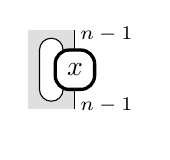
\begin{tikzpicture}[xscale=-1, baseline = -.1cm]
	\fill[shaded] (.6,-.5) -- (.6,.5) -- (0,.5) -- (0,-.5);
	\filldraw[unshaded] (.15,-.25) arc (-180:0:.15cm) -- (.45,.25) arc (0:180:.15cm);
	\draw (0,-.5) -- (0,.5);
	\node at (-.4,.45) {\scriptsize{$n-1$}};
	\node at (-.4,-.45) {\scriptsize{$n-1$}};
	\roundNbox{unshaded}{(0,0)}{.25}{0}{0}{$x$}
\end{tikzpicture}
=
[Y:X]^{-1/2} \sum_{\beta} \beta x\beta^*
$$
where $\{\beta\}$ is a (finite) Pimsner-Popa basis for $X\subset Y$, and this map is independent of the choice of basis.
This means that picking Pimsner-Popa bases $\{\beta\}$ for $X\subset Y$ and $\{b\}$ for $pXp\subset pYp$, we must show that
$$
\Phi_{n-1,-}
\left(
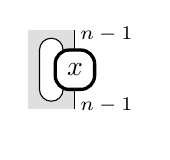
\begin{tikzpicture}[xscale=-1, baseline = -.1cm]
	\fill[shaded] (.6,-.5) -- (.6,.5) -- (0,.5) -- (0,-.5);
	\filldraw[unshaded] (.15,-.25) arc (-180:0:.15cm) -- (.45,.25) arc (0:180:.15cm);
	\draw (0,-.5) -- (0,.5);
	\node at (-.4,.45) {\scriptsize{$n-1$}};
	\node at (-.4,-.45) {\scriptsize{$n-1$}};
	\roundNbox{unshaded}{(0,0)}{.25}{0}{0}{$x$}
\end{tikzpicture}
\right)
=
[Y:X]^{-1/2}p\sum_{\beta} \beta x\beta^* 
= 
[Y:X]^{-1/2}\sum_{b} bpxb^*
=
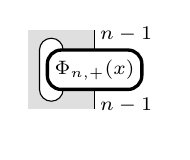
\begin{tikzpicture}[xscale=-1, baseline = -.1cm]
	\fill[shaded] (.85,-.5) -- (.85,.5) -- (0,.5) -- (0,-.5);
	\filldraw[unshaded] (.4,-.25) arc (-180:0:.15cm) -- (.7,.25) arc (0:180:.15cm);
	\draw (0,-.5) -- (0,.5);
	\node at (-.4,.45) {\scriptsize{$n-1$}};
	\node at (-.4,-.45) {\scriptsize{$n-1$}};
	\roundNbox{unshaded}{(0,0)}{.25}{.35}{.35}{\scriptsize{$\Phi_{n,+}(x)$}}
\end{tikzpicture}
.
$$

Now the trick is to carefully choose a Pimsner-Popa basis for $X\subset Y$.
Let $\{b\}$ be a Pimsner-Popa basis for $pXp\subset pYp$, and let $\{a\}$ be a Pimsner-Popa basis for $(1-p)X(1-p) \subset (1-p)Y(1-p)$.
We claim $\{\beta\}=\{a\}\cup \{b\}$ is a Pimsner-Popa basis for $X\subset Y$.
Indeed, we see
$$
\sum_{\beta} \beta e_X \beta^*
=
\sum_{a} ae_X a^* + \sum_{b} be_X b^* 
=
\sum_{a} a(1-p)e_X a^* + \sum_{b} bpe_X b^* 
=
(1-p) + p
= 
1_{\langle Y, e_X\rangle}.
$$
For this special choice of $\{b\}$ and $\{\beta\}$, we immediately see that for $x\in \cP_{n,+}$,
$$
p\sum_{\beta} \beta x\beta^* 
= 
p\left(\sum_{a} ae_X a^* + \sum_{b} be_X b^* \right)
=
\sum_{b} bpe_X b^*
$$
and the result follows.
%
%\nn{please check the following.}
%We carefully choose a Pimsner-Popa basis for $X\subset Y$ as follows.
%First, we pick finitely many partial isometries $v\in p\langle Y, e_X\rangle p$ such that $\sum vv^* = p$ and $v^*v \leq pe_X$.
%Then using the Pimsner-Popa pull-down lemma \nn{}, for each $v$, we get a unique $a\in Y$ such that $ae_X = ve_X$.
%Note that since each $v\in p\langle Y, e_X\rangle p$, the uniqueness of $a\in Y$ immediately implies that $a\in pYp$.
%We now pick finitely many partial isometries $w\in (1-p) \langle Y, e_X\rangle (1-p)$ so that $\sum ww^* = (1-p)$ and $w^*w\leq e_X$.
%Again, we use the pull-down lemma for each $w$ to get a $b\in Y$ with $we_X = be_X$, and we notice that
%$$
%\sum_a ae_X a^* + \sum_b be_X b^* = p + (1-p) = 1_{\langle Y, e_X\rangle},
%$$
%so $\{a\}$ is a Pimsner-Popa basis for $pXp\subset pYp$, and $\{a\}\cup\{b\}$ is a Pimsner-Popa basis for $X\subset Y$.
%
%Now we see that for every $x\in X'\cap Y$, we have
%$$
%p d^{-1}\left( \sum_a axa^* + \sum_b bxb^*\right) = d^{-1}\sum_a a xp a^*,
%$$
%which shows capping on the left commutes with the map $X'\cap Y \ni x \mapsto px \in pX'\cap pYp$.
%The proof for higher left caps is similar.
\end{proof}

%%%%%%%%%%%%%%%%%%%%%%%%%%%%%%%%%%%%%%%%%%%%%%%%%%%%%%%
%%%%%%%%%%%%%%%%%%%%%%%%%%%%%%%%%%%%%%%%%%%%%%%%%%%%%%%
%%%%%%%%%%%%%%%%%%%%%%%%%%%%%%%%%%%%%%%%%%%%%%%%%%%%%%%
\section{The module embedding theorem via towers of algebras}





%%%%%%%%%%%%%%%%%%%%%%%%%%%%%%%%%%%%%%%%%%%%%%%%%%%%%%%
\subsection{Markov sequences}


\begin{defn}
A \emph{Markov sequence} consists of a sequence $(M_n, \tr_n)_{n\geq 0}$ of finite dimensional von Neumann algebras, such that $M_n$ is unitally included in $M_{n_1}$, each $M_n$ has a faithful normal tracial states such that $\tr_{n+1}|_{M_n} = \tr_n$ for all $n\geq 0$, and there is a sequence of \emph{Jones projections} $e_n \in M_{n+1}$ for all $n\geq 1$, such that:
\begin{itemize}
\item
The projections $(e_n)$ satisfy the Temperley-Lieb-Jones relations:
\begin{enumerate}[(1)]
\item
$e_i^2 = e_i = e_i^*$ for all $i$,
\item
$e_i e_j = e_j e_i$ for $|i-j|>1$, and
\item
there is a fixed constant $d>0$ such that $e_{i} e_{i\pm 1} e_i = d^{-2} e_i$ for all $i$.
\end{enumerate}
\item
For all $x\in M_n$, $e_n x e_n = E_n(x)e_n$, where $E_n: M_n \to M_{n-1}$ is the canonical faithful trace-preserving conditional expectation.
\item
For all $n\geq 1$, $E_{n+1}(e_n) = d^{-2}$.
\item
(pull down)
For all $n\geq 1$, $M_{n+1}e_n = M_n e_n$.

\end{itemize}
\end{defn}


\begin{rem}\label{pulldowniff}
$M_n e_n M_n$ is a 2-sided ideal in $M_{n+1}$ for all $n\geq 1$ if and only if the pull down condition holds. Indeed, if the pull down condition holds, then $M_{n+1} M_n e_n M_n \subseteq M_{n+1} e_n M_n = M_n e_n M_n$; the same argument holds on the right by first taking adjoints. Conversely, if $M_n e_n M_n$ is a 2-sided ideal, then $M_{n+1} e_n = (M_{n+1} e_n)e_n \subseteq (M_n e_n M_n) e_n = M_n e_n$.
\end{rem}




\begin{prop}\label{prop:ElementaryMarkov} A Markov sequence satisfies the following elementary properties for $n\geq 1$.
\begin{enumerate}[(A)]
\item
\label{EP:Injective}
The map $M_{n}\ni y\mapsto ye_n \in M_{n+1}$ is injective.

\item
\label{EP:UniquePullDown}
For all $x\in M_{n+1}$, $d^{2}E_{n+1}(x e_n)$ is the unique element $y\in M_n$ such that $x e_n = ye_n$ \cite[Lem.~1.2]{MR860811}.

\item
\label{EP:MarkovTraces}
The traces $\tr_{n+1}$ satisfy the following \emph{Markov property} with respect to $M_n$ and $e_n$: for all $x\in M_n$, $\tr_{n+1}(xe_n) = d^{-2} \tr_n(x)$.

\item
\label{EP:CompressM_{n+1}}
$e_n M_{n+1}e_n = M_{n-1}e_n$.

\item
\label{EP:2SidedIdeal}
$X_{n+1}:=M_n e_n M_n$ is a 2-sided ideal of $M_{n+1}$, and thus $M_{n+1}$ splits as a direct sum of von Neumann algebras $X_{n+1}\oplus Y_{n+1}$.
(In \cite[Thm.~4.1.4 and Thm.~4.6.3]{MR999799}, $Y_{n+1}$ is the so-called `new stuff'.)
By convention, we define $Y_0 = M_0$ and $Y_1 = M_1$, so that $X_0 = (0)$ and $X_1 = (0)$.

\item
\label{EP:BasicContruction}
The map $ae_n b\mapsto ap_n b$ gives a $*$-isomorphism from $X_{n+1}=M_n e_n M_n$ to $\langle M_n , p_n\rangle=M_np_nM_n$, the Jones basic construction of $M_{n-1} \subseteq M_n$ acting on $L^2(M_n,\tr_n)$.

\item
\label{EP:OtherMarkovDef}
Under the isomorphism $X_{n+1} \cong M_n p_n M_n$, the canonical non-normalized trace $\Tr_{n+1}$ on the Jones basic construction algebra $M_np_nM_n$ satisfying $\Tr_{n+1}(ap_nb) = \tr_n(ab)$ for $a,b\in M_n$ equals $d^2 \tr_{n+1}|_{X_{n+1}}$.

\item
\label{EP:NewStuff}
If $y\in Y_{n+1}$ and $x\in X_{n}$, then $yx = 0$ in $M_{n+1}$.
Hence $E_{n+1}(Y_{n+1}) \subseteq Y_{n}$.
(``The new stuff comes only from the old new stuff" \cite{MR999799}.)

\item
\label{EP:FiniteDepth}
If $Y_n =(0)$, then $Y_{k} = (0)$ for all $k\geq n$.

\end{enumerate}
\end{prop}

\begin{proof} 

\begin{enumerate}[(A)]
\item\label{inj}

We know that $d^2E_{n+1}(ye_n) = y $, so the proposed map has a left inverse.

\item

This follows directly from \eqref{inj}

\item

For $x\in M_n$, we have $\tr_{n+1}(xe_n) = \tr_n(E_{n+1}(xe_n)) = \tr_n(x E_{n+1}(e_n)) = d^{-2} \tr_n(x)$, since $E_{n+1}(e_n) = d^{-2}$.

\item

$M_{n+1} e_n = M_n e_n$ and $e_nxe_n = E_n(x)e_n$ for all $x\in M_n$.

\item

$M_ne_nM_n$ is a 2-sided ideal of $M_{n+1}$ by the pull down condition, as discussed in \eqref{pulldowniff}

\item

% It suffices to show the map is injective, which shows it is well-defined. % This was written here, but I can't make sense of it. 
First, we check that the map $\phi:ae_nb\to ap_nb$ is injective. 
Suppose $\sum a_i p_n b_i = 0$.
Then for all $a,b\in M_n$, we have $0=p_na\left(\sum a_i p_n b_i\right) bp_n = \sum E_{n}(aa_i)E_n(b_ib)p_n$, and therefore $\sum E_{n}(aa_i)E_n(b_ib) = 0$ as $M_n \ni x\mapsto xp_n \in \langle M_n, p_n\rangle$ is injective.
Hence $$0 = \sum E_{n}(aa_i)E_n(b_ib)e_n = e_na\left(\sum a_i e_n b_i\right) be_n$$ for all $a,b\in M_n$, and thus $\sum a_i e_n b_i = 0$, so $\phi$ is injective. 

		To show that $\phi$ is well-defined, we may reverse the above argument, using \eqref{EP:Injective}. 
		It is clear that $\phi$ is surjective. 

\item

For $a,b\in M_n$, we have 
$\Tr_{n+1}(ap_n b) = \tr_n(ab) = \tr_n(ba) = d^2\tr_{n+1}(bae_n) = d^2 \tr_{n+1}(ae_n b)$.

\item

Since $X_0 = (0)$ and $X_1 = (0)$ by definition, we may assume $n\geq 2$.
As in the proof of \cite[Thm.~4.6.3.vi]{MR999799}, we may assume $y$ is a central projection in $M_{n+1}$ such that $y e_{n} = 0$.
Then for all $ae_{n-1} b \in X_n$, $y ae_{n-1} b = d^2 yae_{n-1} e_{n}e_{n-1} b = d^2 ae_{n-1} ye_{n} e_{n-1} b = 0$.
The final claim follows from $z_{n}E_{n+1}(y) = E_{n+1}(z_n y)= 0$ where $z_n$ is the central support of $e_{n-1}$ in $M_n$.

\item

This follows immediately from the previous fact.

\end{enumerate}

\end{proof}


Notice that by \eqref{EP:BasicContruction}, the Bratteli diagram for the inclusion $M_{n}\subset M_{n+1}$ consists of the reflection of the Bratteli diagram for the inclusion $M_{n-1} \subset M_n$, together with possibly some new edges and vertices corresponding to simple summands of $Y_{n+1}$. By \eqref{EP:NewStuff}, the new vertices at level $n+1$ only connect to the vertices that were new at level $n$. This leads to the following definition:


\begin{defn}
The \emph{principal graph} of the Markov sequence $(M_n,\tr_n)$ with Jones projections $(e_n)$ consists of the \emph{new} vertices at every level $n$ of the Bratteli diagram, together with all the edges connecting them.

A Markov sequence is said to have \emph{finite depth} if the principal graph is finite.
\end{defn}


It follows that a Markov sequence has finite depth if and only if there is $n\in \bbN$ such that $Y_n = (0)$, as in \ref{prop:ElementaryMarkov} \eqref{EP:FiniteDepth}. Let $(M_n)$ be a Markov sequence with finite depth, and take the minimal integer $n\in \bbN$ such that $Y_n=(0)$. Now notice that for $k<n$ the Bratteli diagram of $M_k\subseteq M_{k+1}$ is the Bratteli diagram of $M_{k-1}\subseteq M_{k}$ reflected upwards along with additional edges which are part of the principal graph. Because of this and the fact that the Bratteli diagram for $M_0\subseteq M_1$ is part of the principal graph we can ``unravel" the Bratteli diagram for $M_{n}\subseteq M_{n+1}$ to obtain the principal graph for the Markov sequence $(A_n,\tr_n)$.

\begin{fact}\label{BratteliPrincipal}
	If a Markov sequence $(M_n)$ has finite depth and $n\in \bbN$ is such that $Y_n=(0)$, then for $k\geq n$, there is a canonical graph isomorphism between the principal graph of $(M_n)$ and the Bratteli diagram for $M_{k}\subset M_{k+1}$.
\end{fact}

\begin{ex}
The Temperley-Lieb algebras of modulus $d\geq 2$ with the usual Jones projections form a Markov sequence. Their principal graph is $A_{\infty}$.
\end{ex}

%%%%%%%%%%%%%%%%%%%%%%%%%%%%%%%%%%%%%%%%%%%%%%%%%%%%%%%
\subsection{Planar algebras and the paragroup}  \label{cattheory}
\nn{find a new home for me.}

Planar algebras were originally introduced in \cite{planaralg1}. We will use the same definitions and conventions as \cite{penneys}, \cite{peters}, \cite{jones}, and \cite{planaralg2}. The reader is referred to these references for further information on planar algebras. From any subfactor planar algebra, one may construct a 2-category. We refer the reader to \cite{paragroup} and \cite{paragroup2} for more details. We adopt the definitions used in \cite{paragroup}, since we wish to work with shaded planar algebras.

\begin{defn}\textnormal{
		Let $Q_{\bullet}$ be a subfactor planar algebra. The \textit{paragroup} of $Q_\bullet$ is a 2-category $\cG$: 
\begin{itemize}
\item The 0-morphisms of $\cG$ are the two objects
$\uscircle$ and $\scircle$.
\item The 1-morphisms are projections in the box spaces of $Q_{\bullet}$, as follows:
\begin{itemize}
	\item $\Hom_{\cG}(\uscircle\rightarrow\uscircle)=\{p\in Q_{i,+}|\text{$p$ is projection and $i$ is even}\}$
	\item $\Hom_{\cG}(\uscircle\rightarrow\scircle)=\{p\in Q_{i,+}|\text{$p$ is projection and $i$ is odd}\}$
	\item $\Hom_{\cG}(\scircle\rightarrow\uscircle)=\{p\in Q_{i,-}|\text{$p$ is projection and $i$ is odd}\}$
	\item $\Hom_{\cG}(\scircle\rightarrow\scircle)=\{p\in Q_{i,-}|\text{$p$ is projection and $i$ is even}\}$
\end{itemize}
Composition of $1$-morphisms is denoted by $\otimes$ and represented diagrammatically by horizontal concatenation of diagrams.
\item The 2-morphisms of $\cG$ are defined as follows: for $p\in P_{i,\pm}$ and $q\in P_{i,\pm}$, we set $\Hom_{\cG}(p\rightarrow q)=qP_{j\rightarrow i}p$. The space $P_{j\rightarrow i}$ is just $P_{i+j}$, except that tangles are depicted with $j$ with strings emanating from the top and $i$ from the bottom. Note that by construction, $i+j$ is always even. 
\end{itemize}}
\end{defn}

For a general subfactor planar algebra $Q_{\bullet}$, the $2$-category $\cG$ can be interpreted as a unitary multitensor category $\cC$ with the canonical spherical unitary dual functor following \cite{egno,UnitaryDualFunctors}. 
When $Q_{\bullet}$ is finite depth, $\cC$ is a $2\times 2$ unitary multifusion category. 

By a module over $Q_\bullet$, we mean a $\ast$-module category over the $\ast$-multitensor category $\cC$. Let $\cM$ be a cyclic left $\cC$-module category with generator $m$. 
Since $\cM$ is indecomposable, we can take $m$ to be simple. 
By \cite{ostrik03}, there is a $\ast$-algebra $A$ internal to $\cC$ such that $\cM\cong\FreeMod_\cC(A)$, the category of free right $A$-modules internal to $\cC$, namely the $\cC$-valued internal $\End$ of $m$. 
Since $m$ is simple, 
$A$ is in fact a Q-system, % Q-system or $Q$-system?
as described in \cite[Rmk.2.7]{ny17}.  
Each module in this category is of the form $X\otimes A$ for some $X\in\cC$. 
Each $X$ in $\cC$ is trivially a bimodule over the tensor unit $1_{0,+}\oplus1_{0,-}$, so each $X\in\Irr(\cC)$ is a module over either $1_{0,+}$ or $1_{0,-}$ on each side. 
We can therefore view $\cG$ as the $2$-category of bimodules over the algebra objects $1_{0,+}$ and $1_{0,-}$ and view $\cM$ as the category of $1_{0,+}-A$ and $1_{0,-}-A$ bimodules. 
By \cite[Thm.4.1]{ny17}, we can again obtain a $3\times 3$ unitary multifusion category $\widetilde{\cC}$ from the $2$-category of bimodules over the algebras $1_{0,+}$, $1_{0,-}$, and $A$, into which both $\cC$ and $\cM$ have naturally monoidal embeddings. 
Taking the full subcategory of objects which are preserved by tensoring by the appropriate components of the tensor unit allows us to recover a $2\time 2$ multifusion subcategory $\cC$ and a cyclic $\cC$-module $\cM$. 



%%%%%%%%%%%%%%%%%%%%%%%%%%%%%%%%%%%%%%%%%%%%%%%%%%%%%%%
%\section{Construction of the Planar Algebra Associated to a Module Category}
\subsection{Constructing a Markov sequence}
Given a finite depth subfactor planar algebra $Q_{\bullet}$ and a module $\cM$ over $Q_{\bullet}$, let $\cC$ and $\widetilde{\cC}$ be the multifusion categories associated to $\cG$ and $\cM$, as described in section \ref{cattheory}. Let $1_{\widetilde{\cC}}= 1_0 \oplus 1_1 \oplus 1_2$ be the tensor unit in $\widetilde{\cC}$, indexed so that $\cC$ is the non-unital $2\times 2$ unitary multifusion subcategory of $\widetilde{\cC}$ with $1_\cC = 1_0\oplus 1_1$, and $\cM\cong\cC_{20}\oplus \cC_{21}$. Overall,
$$
\cM 
=
\begin{pmatrix}
\cC_{20} & \cC_{21} 
\end{pmatrix}
\qquad\qquad
\cC
=
\begin{pmatrix}
\cC_{00} & \cC_{01} 
\\
\cC_{10} & \cC_{11}
\end{pmatrix}
\subset
\begin{pmatrix}
\cC_{00} & \cC_{01} & \cC_{02}
\\
\cC_{10} & \cC_{11} & \cC_{12}
\\
\cC_{20} & \cC_{21} & \cC_{22}
\end{pmatrix}
=
\widetilde{\cC}
$$
Let $x\in \cC_{01}$ be the strand pictured below:
$$x=

\begin{tikzpicture}[baseline=-.1cm]
	\fill[white] (0,-.7) rectangle (-.7,-.7);
	\fill[shaded] (0,-.7) rectangle (.7,.7);
	\draw (0,-.7) -- (0,.7);

\end{tikzpicture}
\ \,\,\,\,\, \text{and,}\,\,\,\,\, \overline{x}=

\begin{tikzpicture}[baseline=-.1cm]
	\fill[white] (0,-.7) rectangle (.7,.7);
	\fill[shaded] (0,-.7) rectangle (-.7,.7);
	\draw[fill] (0,-.7) -- (0,.7);

\end{tikzpicture}
\,\,\,\,\, \text{so} \,\,\,\,\, x\otimes \overline{x} = 
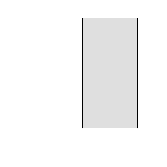
\begin{tikzpicture}[baseline=-.1cm]
	\fill[white] (0,-.7) rectangle (-.7,.7);
	\fill[shaded] (0,-.7) rectangle (.7,.7);
	\draw (0,-.7) -- (0,.7);
	\draw (.7,-.7) -- (.7,.7);

\end{tikzpicture}
$$
By construction, $x$ is a generating object for $\cC$. If we pick a simple object $m\in \cC_{20}$, since $\cM$ is indecomposable, we have that any object of $\cM$ is isomorphic to a direct summand of $m\otimes \xalt$ for some nonnegative integer $n$, where $$
x^{\text{alt}\otimes n}:=\underbrace{x\otimes \overline{x} \otimes x \otimes \cdots \otimes x^?}_{n \text{ tensorands}}\,,
$$ and $x^? = \overline x$ if $n$ is even and $x$ if $n$ is odd. We define $\xbaralt$ similarly.

We will construct a finite depth Markov sequence of algebras from the action of $\cC$ on $\cM$ as follows. Set $A_n=\End_{\widetilde{\cC}}(m\otimes \xalt)$. We can represent morphisms in $A_n$ as 
$$
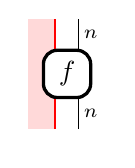
\begin{tikzpicture}[baseline=-.1cm]
	\fill[ctwoshading] (-.15,-.7) rectangle (-.5,.7);
	\draw[thick, red] (-.15,-.7) -- (-.15,.7);
	\draw (.15,-.7) -- (.15,.7);
	\roundNbox{unshaded}{(0,0)}{.3}{0}{0}{$f$}
	\node at (.3,.5) {\scriptsize{$n$}};
	\node at (.3,-.5) {\scriptsize{$n$}};
\end{tikzpicture}
$$
where the red strand represents $m$ and the $n$ represents $x^{\text{alt}\otimes n}$. We have a faithful tracial state $\tr_n:A_n\to \C$ given by
\begin{equation}\label{eq:TraceAn}
\tr_n(f) 
\,:=\, 
\frac{1}{\dim_{\widetilde{\cC}}(m)\dim_{\widetilde{\cC}}(x)^n}\cdot\tr_{\widetilde{\cC}}(f)
\,=\,
\frac{1}{\dim_{\widetilde{\cC}}(m)}\cdot
\frac{1}{d^n}
\cdot
\left(
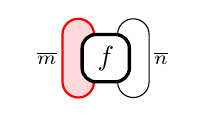
\begin{tikzpicture}[baseline=-.1cm, rotate=90]
	\filldraw[thick, red, ctwoshading] (-.3,.15) arc (270:90:.2cm) -- (.3,.55) arc (90:-90:.2cm);
	\draw (-.3,-.15) arc (90:270:.2cm) -- (.3,-.55) arc (-90:90:.2cm);
	\roundNbox{unshaded}{(0,0)}{.3}{0}{0}{$f$}
%	\node at (-.7,-.35) {\scriptsize{$n$}};
	\node at (0,-.7) {\scriptsize{$\overline{n}$}};
	\node at (0,.75) {\scriptsize{$\overline{m}$}};
%	\node at (.7,.35) {\scriptsize{$m$}};
\end{tikzpicture}
\right)
\end{equation}
Where $n$ and $\overline{n}$ represent $\xalt$ and $\xbaralt$, respectively. This makes each $A_n$ a finite dimensional von Neumann algebra.

\begin{rem}
	The trace can be identified with a complex scalar because $\overline{m}\otimes m\in\cC_{00}$, the red cup $1\to\overline{m}\otimes m$ and cap $\overline{m}\otimes m\to 1$ factor through the simple summand $1_0$. Since $1_0\otimes 1\cong 1_0$, the trace is a member of the $1$-dimensional algebra $\End_{\widetilde{\cC}}(1_0)\subseteq\End_{\widetilde{\cC}}(1)$. 
\end{rem}

We also have a natural tracial inclusion $A_n \rightarrow A_{n+1}$ % such that the trace restricts ($tr_{n+1}|_{A_n}=tr_n$):
\begin{equation}\label{eq:Inclusion}
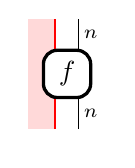
\begin{tikzpicture}[baseline=-.1cm]
	\fill[ctwoshading] (-.15,-.7) rectangle (-.5,.7);
	\draw[thick, red] (-.15,-.7) -- (-.15,.7);
	\draw (.15,-.7) -- (.15,.7);
	\roundNbox{unshaded}{(0,0)}{.3}{0}{0}{$f$}
	\node at (.3,.5) {\scriptsize{$n$}};
	\node at (.3,-.5) {\scriptsize{$n$}};
\end{tikzpicture}
\mapsto
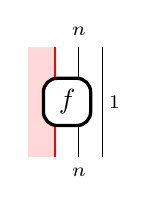
\begin{tikzpicture}[baseline=-.1cm]
	\fill[ctwoshading] (-.15,-.7) rectangle (-.5,.7);
	\draw[thick, red] (-.15,-.7) -- (-.15,.7);
	\draw (.15,-.7) -- (.15,.7);
	\draw (.45,-.7) -- (.45,.7);
	\roundNbox{unshaded}{(0,0)}{.3}{0}{0}{$f$}
	\node at (.15,.9) {\scriptsize{$n$}};
	\node at (.15,-.9) {\scriptsize{$n$}};
	\node at (.6,0) {\scriptsize{$1$}};
\end{tikzpicture}
\end{equation}
and a trace preserving conditional expectation $E_n:A_n\rightarrow A_{n-1}$, 
\begin{equation}\label{eq:ConditionalExpectationAn}
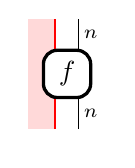
\begin{tikzpicture}[baseline=-.1cm]
	\fill[ctwoshading] (-.15,-.7) rectangle (-.5,.7);
	\draw[thick, red] (-.15,-.7) -- (-.15,.7);
	\draw (.15,-.7) -- (.15,.7);
	\roundNbox{unshaded}{(0,0)}{.3}{0}{0}{$f$}
	\node at (.3,.5) {\scriptsize{$n$}};
	\node at (.3,-.5) {\scriptsize{$n$}};
\end{tikzpicture}
\mapsto\,
\frac{1}{d}
\cdot
\left(\,\,
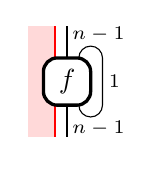
\begin{tikzpicture}[baseline=-.1cm]
	\fill[ctwoshading] (-.15,-.7) rectangle (-.5,.7);
	\draw[thick, red] (-.15,-.7) -- (-.15,.7);
	\draw (0,-.7) -- (0,.7);
	\draw (.15,.3) arc (180:0:.15cm) -- (.45,-.3) arc (0:-180:.15cm);
	\roundNbox{unshaded}{(0,0)}{.3}{0}{0}{$f$}
	\node at (.4,.6) {\scriptsize{$n-1$}};
	\node at (.4,-.6) {\scriptsize{$n-1$}};
	\node at (.6,0) {\scriptsize{$1$}};
\end{tikzpicture}
\right)
\end{equation}
left inverse to the inclusion.

Here, $d:=\dim_{\widetilde{\cC}}(x)=\dim_{\widetilde{\cC}}(\overline{x})$ the value of a closed loop appearing in the diagram. % There must be a better word for this. Maybe we should also remark why these are equal? In response: Emily peter's uses the term closed circles (on page 7 of her thesis), if that's the woridng you mean, and the equality follows from sphericality, maybe we should this should probably be in the preliminary discussion of the paragroup and the constructed multifusion category
Given the previously defined inclusion and that multiplication is given by vertical stacking of diagrams, it's clear that $E_n$ is $A_{n-1}$ bilinear. Similarly, we have that $tr_n=tr_{n-1} \circ E_n$.

Finally, the Jones projections for each inclusion $A_{n}\subset A_{n+1}$ are given by
\begin{equation}\label{eq:JonesProjections}
e_n
:=
\frac1d\cdot
\left(\,\,
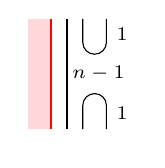
\begin{tikzpicture}[baseline=-.1cm]
	\fill[ctwoshading] (-.3,-.7) rectangle (-.6,.7);
	\draw[thick, red] (-.3,-.7) -- (-.3,.7);
	\draw (-.1,-.7) -- (-.1,.7);
	\draw (.1,-.7) -- (.1,-.4) arc (180:0:.15cm) -- (.4,-.7);
	\draw (.1,.7) -- (.1,.4) arc (-180:0:.15cm) -- (.4,.7);
%	\node at (-.1,-1) {\scriptsize{$n-1$}};
	\node at (.3,0) {\scriptsize{$n-1$}};
	\node at (.6,.5) {\scriptsize{$1$}};
	\node at (.6,-.5) {\scriptsize{$1$}};
\end{tikzpicture}
\right)
\in
A_{n+1}.
\end{equation}
where the $n-1$ indicates $n-1$ vertical strands with appropriate shading to the right of the red strand. The Temperley-Lieb- % strange editor enforced wordwrap from here. lint?
Jones relations follow immediately from the definition and the fact that closed loops count for a factor of $d$. Similarly, 
for any $x\in A_n$ we have $e_nxe_n=E_n(x)e_n$. Clearly, $E_{n+1}(e_n)=d^{-2}\id_{m \otimes \xalt}$. Finally, the pull 
down condition holds, as for each $x\in A_{n+1}$, we have that $d^2 E_{n+1}(xe_n)e_n=xe_n$. Equivalently, $A_{n} e_n A_n$ is a 
two-sided ideal in $A_{n+1}$. Thus, the tower algebras given by the $A_n$ is indeed a Markov sequence.
 
\begin{prop}
The Markov sequence of von Neumann Algebras $\left(A_n, tr_n\right)_{n\geq 0}$ is finite depth.
\end{prop}

\begin{proof}
	When $n$ is even, we have:
	\[m\otimes \xalt \cong \bigoplus\limits_{Y\in\Irr(\cC_{20})}\left(n_YY\right) \]
 For some nonnegative integers $n_Y$. Therefore, 
	\[\End_{\widetilde{\cC}}\left(m\otimes\xalt\right)\cong \bigoplus\limits_{Y\in \Irr(\cC_{20})}\End_{\widetilde{\cC}}\left(n_Y Y\right) \]
	The case when $n$ is odd is similar. This means that the Bratteli diagram for $A_n\subseteq A_{n+1}$ has at most $|\Irr(\cC_{20})|+|\Irr(\cC_{21})|$ vertices, so the principal graph must be finite. 
\end{proof}

\begin{thm}
The principal graph obtained from the Markov sequence $\left(A_n, tr_n\right)_{n\geq 0}$ is independent of the choice of $m$, and is in fact isomorphic to the fusion graph for the action of $x$ on $\cM$.
\end{thm}

\begin{proof}
Because $x$ generates $\cC$ and $\cM$ is cyclic, we can assume that every simple object in $\cM$ is a direct summand of $m\otimes \xalt $. Essentially, our result from the fact that subsequent in inclusions $A_k\subseteq A_{k+1}$ are given by tensoring $\id_x$ and $\id_{\overline{x}}$, so they are determined entirely by the fusion rules.

First, recall that for a finite depth Markov sequence, the principal graph is canonically isomorphic to the Bratteli for the inclusion $A_n\subseteq A_{n+1}$ for $n$ large enough by \ref{BratteliPrincipal}. So, it suffices to show this Bratteli diagram is isomorphic to the fusion graph for $\cM$. Furthermore if $n$ is such that $A_n\subseteq A_{n+1}\subseteq A_{n+2}$ is standard then for $k\geq n$ the Bratteli diagram for $A_{k}\subseteq A_{k+1}$ is isomorphic to the Bratteli diagram for $A_n\subseteq A_{n+1}$, so without loss of generality, we may assume that $n$ is even.

Let the non-negative integers $p_{Z,Y}$ be defined by the following equation:
	\[Y\otimes x\cong\bigoplus\limits_{\Irr(\cC_{21})}\left(p_{Z,Y}Z\right)\]
These coefficients are exactly the coefficients for the adjacency matrix of the fusion graph for $x$ acting on $\cM$.

Recall that
$$A_n=\End_{\widetilde{\cC}}\left(m\otimes\xalt\right)\cong \bigoplus\limits_{\Irr(\cC_{20})}\End_{\widetilde{\cC}}\left(n_Y Y\right)$$
where 
$$m \otimes \xalt \cong \bigoplus\limits_{\Irr(\cC_{20})}\left(n_YY\right)$$
	Note that we may choose $n$ such that each $n_Y$ is strictly positive, as there is some $n$ such that $\bigoplus\limits_{\Irr(\cC_{20})}Y$ is isomorphic to a direct summand of $m\otimes \xalt$. (In fact, the first $n$ where this happens is exactly when the Markov sequence achieves depth.) % Strictly speaking, this is not true, because the Markov sequence may first achieve depth when $n$ is odd. But going into that may not clarify the proof. 

The inclusion of $A_n \hookrightarrow A_{n+1}$ is given by $\phi \mapsto \phi \otimes \id_{x}$. Each $\phi \in A_n$ is uniquely defined as a direct sum \[\bigoplus\limits_{\Irr(\cC_{20})}\phi_Y\]
where each $\phi_Y \in \End_{\widetilde{\cC}}\left(n_YY\right)$. Then, distributing tensor products over the sum, we may write $\phi$ as 
	\[\bigoplus_{\Irr(\cC_{20})}\left(\phi_Y \otimes \id_{x}\right)\]
But then:
	\[\phi_Y \otimes \id_{x} \in \End_{\widetilde{\cC}}\left(n_Y Y \otimes x\right)\cong \bigoplus\limits_{\Irr({\cC}_{21})} \End_{\widetilde{\cC}}\left( p_{Z,Y} n_Y Z\right)\]
Since all $n_j\neq 0$ and the inclusion is unital, it is clear that $p_{Z,Y}$ gives the coefficients for the Bratteli diagram.
\end{proof}



%%%%%%%%%%%%%%%%%%%%%%%%%%%%%%%%%%%%%%%%%%%%%%%%%%%%%%%
\subsection{The Embedding Theorem}

\begin{claim*}
A finite depth subfactor planar algebra can be embedded into the bipartite graph planar algebra of the fusion graph of the right action of the strand on a cyclic module.
\end{claim*}
As described in \cite{penneys}, one can define a canonical shaded planar $*$-algebra structure on the tower of relative commutants of the base of a strongly Markov tower of algebras. % Now that this construction is summarized in a subsection of section 2, we may want to shorten this reference to there. 
This planar algebra is isomorphic to the bipartite graph planar algebra of the Bratteli diagram of the first inclusion in the tower, by theorem 3.28 of \cite{penneys}. We have shown that the Markov sequence $(A_n,\tr_n)$ defined in the previous section is finite depth. Let $r$ be the minimal integer such that the inclusion $A_{2r} \subset A_{2r+1} \subset A_{2r+2}$ is standard, and let $B_n=A_{2r+n}$. Then the canonical planar $*$-algebra $P_\bullet$ associated to $B_0\subseteq (B_1,tr_1)$ is isomorphic to the bipartite graph planar algebra of the principle graph of the tower $\left(A_{n}\right)$; indeed, by fact \ref{BratteliPrincipal}, the principle graph of $(A_{n},tr_n)$ is isomorphic to the Bratteli diagram of $B_0\subseteq B_1$.
If we denote the canonical $*$-planar algebra associated to $B_0\subseteq(B_1,tr_1)$ by $P_{\bullet}$, then by construction, we have the following:
\begin{align*}
	P_{n,+} &=  A'_{2r}\cap A_{2r+n} \\
	P_{n,-}  &= A'_{2r+1}\cap A_{2r+n+1} 
\end{align*}

Consider the map $\Phi$, which places $2r$ strings to the left of elements in $Q_{n,+}$  and $2r+1$ strings to the left of elements in $Q_{n,-}$:
\[ 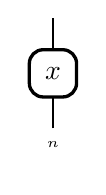
\begin{tikzpicture}[baseline]
	\draw (0,-.7) -- (0,.7);
	\roundNbox{unshaded}{(0,0)}{.3}{0}{0}{$x$}
	\node at (0,-.9) {\tiny{$n$}};
\end{tikzpicture}
\quad
\begin{tikzpicture}[baseline]
	\clip (0.5,0.9) -- (-0.5,0.9) -- (-0.5,-0.9) -- (0.5,-0.9);
	\draw [|->,thick] (-0.3,0)--(0.3,0);
	\node at (0,0.25) {\scriptsize{$\Phi$}};
\end{tikzpicture}
\quad
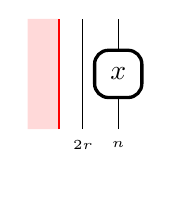
\begin{tikzpicture}[baseline]
	\fill[ctwoshading] (-.3,-.7) -- (-0.3,.7) -- (-.7,0.7) -- (-.7,-0.7) -- (-.3,-0.7);
	\draw[thick,red] (-0.3,-.7) -- (-0.3,0.7);
	\draw (0.45,-.7) -- (0.45,.7);
	\draw (0,-.7) -- (0,.7);
	\roundNbox{unshaded}{(0.45,0)}{.3}{0}{0}{$x$}
	\node at (0.45,-.9) {\tiny{$n$}};
	\node at (0,-0.9){\tiny{$2r$}};
\end{tikzpicture} \]
This map sends $Q_{n , +}$ to $P_{n,+}$ and $Q_{n , -}$ to $P_{n,-}$. In order to check that $\Phi(Q_{\bullet})$ is a planar $\ast$-subalgebra, we use lemma 2.48 in \cite{penneys}.
We shall state it here for the reader's convenience:
\begin{lem}[Preservation under action of tangles]
Suppose that $P_\bullet$ is a planar $\ast$-algebra with modulus $d \neq 0$ and $Q_{n,\pm} \subset P_{n,\pm}$ are $\ast$-subalgebras which are preserved by the action of the following tangles:

\begin{enumerate}[(1)]
\item Multiplication by tangles of the form $E_n = 
\begin{tikzpicture}[baseline]
	\draw (-.1,-.7) -- (-.1,.7);
	\draw (.5,-.7) -- (.5,-.4) arc (180:0:.15cm) -- (.8,-.7);
	\draw (.5,.7) -- (.5,.4) arc (-180:0:.15cm) -- (.8,.7);
%	\node at (-.1,-1) {\scriptsize{$n-1$}};
	\node at (-.1,-.9) {\tiny{$n-1$}};
\end{tikzpicture}
$
\item 
\begin{enumerate}[(i)]
\item (Right Capping) $\alpha_n = 
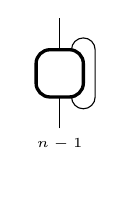
\begin{tikzpicture}[baseline]
	\draw (0,-.7) -- (0,.7);
	\draw (.15,.3) arc (180:0:.15cm) -- (.45,-.3) arc (0:-180:.15cm);
	\roundNbox{unshaded}{(0,0)}{.3}{0}{0}{}
	\node at (0,-0.9) {\tiny{$n-1$}};
\end{tikzpicture}
: P_{n,+} \to P_{n-1,+}
$
\item (Inclusion) $\beta_n = 
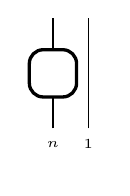
\begin{tikzpicture}[baseline]
	\draw (0,-.7) -- (0,0.7);
	\draw (0.45,-.7) -- (0.45,.7);
	\roundNbox{unshaded}{(0,0)}{.3}{0}{0}{}
	\node at (0,-.9) {\tiny{$n$}};
	\node at (0.45,-.9) {\tiny{$1$}};
\end{tikzpicture}
: P_{n,+} \to P_{n+1,+}
$
\item (Left Capping) $\gamma^{+}_n =
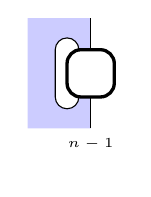
\begin{tikzpicture}[baseline]
	\fill[relativecommutantshading] (0,-.7) -- (-.8,-.7) -- (-.8,.7) -- (0,.7) -- (0,-.7);
	\fill[unshaded] (-.15,.3) arc(0:180:.15cm) -- (-.45,-.3)arc(-180:0:0.15cm)--(-.15,.3);
	\draw (0,-.7) -- (0,.7);
	\draw (-.15,.3) arc (0:180:.15cm) -- (-.45,-.3) arc (-180:0:.15cm);
	\roundNbox{unshaded}{(0,0)}{.3}{0}{0}{}
	\node at (0,-0.9) {\tiny{$n-1$}};
\end{tikzpicture}
: P_{n,+} \to P_{n-1,-}
$ 
\end{enumerate}
\item (Left inclusion) $i^{-}_n =
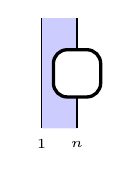
\begin{tikzpicture}[baseline]
	\fill[relativecommutantshading] (-0.45,.7) -- (0,.7) -- (0,-.7) -- (-0.45,-.7) -- (-0.45,.7);
	\draw (0,-.7) -- (0,0.7);
	\draw (-0.45,-.7) -- (-0.45,.7);
	\roundNbox{unshaded}{(0,0)}{.3}{0}{0}{}
	\node at (0,-.9) {\tiny{$n$}};
	\node at (-0.45,-.9) {\tiny{$1$}};
\end{tikzpicture}
: P_{n,-} \to P_{n+1,+}
$ 
\end{enumerate}
Then the $Q_{n,\pm}$ are preserved under every tangle and thus form a planar $\ast$-subalgebra $Q_\bullet \subset P_\bullet$
\end{lem}

We denote traces in $Q_{\bullet}$ by $\overline{\tr}$ and traces in $P_{\bullet}$ by $\tr$. We denote the Jones projections in $Q_{\bullet}$ by $E_{j}$ and the Jones projections in  $P_{\bullet}$ by $F_{j}$.


\begin{thm}
The image of the map $\Phi:Q_{\bullet} \to P_{\bullet}$ is a $\ast$-planar subalgebra of $P_{\bullet}$.
\end{thm} 

\begin{proof}
Observe that for all $x,y \in Q_{\bullet}$, we have that 
\begin{align}
	\Phi(x^{*}) &= \Phi(x)^{\ast} \\
	\Phi(xy) &= \Phi(x)\Phi(y) \\
	\overline{\tr}_{n}(x) &= \frac{1}{\dim_\cC(x)^{2r}}\cdot\tr_{n}(\Phi(x)) \label{eq3}
\end{align}

	To prove the injectivity of $\Phi$, we can use the faithfulness of the traces and equation \eqref{eq3}.
	In section \ref{ssec:canonical}, we see % do we? Perhaps enhance the section appropriately or add another subsection
	that in the relative commutant planar algebra, the tangles described in Lemma 2.48 are associated to known functions. Thus, we can check that $\Phi(Q_\bullet)$ is preserved under the specified tangles by using both algebraic and pictorial relations. We now proceed to check the requirements of Lemma 2.48:
\begin{enumerate}[(1)]
\item By the construction of $P_{\bullet}$, we know that $\Phi(E_j)=F_j$. Thus, $\Phi(Q_{n,\pm})$ is closed under multiplication by Jones projections. 
\item \begin{enumerate}[(i)]
\item \label{condex} Clearly, $\Phi(\alpha_n(x)) = \alpha_{2r+n}(\Phi(x))$.
\item Similarly to \eqref{condex}, it is clear that $\Phi(\beta_n(x)) = \beta_{2r+n}(\Phi(x))$. In fact, the inclusion from $P_{n,+} \to P_{n+1,+}$ is just the restriction of the inclusion from $Q_{2r+n,+} \to Q_{2r+n+1,+}$. 
\item In section \ref{ssec:canonical}, % maybe cite definition. % maybe expand the explanation of the definitio, to make the claim about $\gamma_n$ clear
 we showed that the left-capping tangle $\gamma_n$ in the canonical planar $\ast$-algebra is given by 
\[
 \gamma^{+}_n(x) = \frac{1}{d^2}\sum_{b \in B}bxb^\ast
\]
where $B$ is a Pimnser Popa basis of $B_1$ over $B_0$. We will now check that $\gamma^{+}_n$ preserves $\Phi(Q_{\bullet})$. 
		For any $x \in Q_{n,+}$, we have 

\centerline{
  \begin{minipage}{\linewidth}
			\[
				d^2\gamma^+_n(\Phi(x))
				=
\sum_{b\in B}
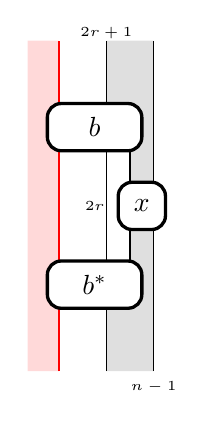
\begin{tikzpicture}[baseline]
	\fill[ctwoshading] (-1,-2.1) -- (-1,2.1) -- (-.6,2.1) -- (-.6,-2.1) -- (-1,-2.1);
	\fill[shaded] (0,2.1) -- (0,0.7) -- (0.3,0.7) -- (0.3,-0.7) -- (0,-0.7) -- (0,-2.1) -- (0.6,-2.1) -- (0.6,2.1) -- (0,2.1);
	\draw[thick,red] (-0.6,-2.1) -- (-0.6,2.1);
	\draw (0.6,-2.1) -- (0.6,2.1);
	\draw (0.3,-.7) -- (0.3,.7);
	\draw (0,-2.1) -- (0,2.1);
	\roundNbox{unshaded}{(0.45,0)}{.3}{0}{0}{$x$}
	\roundNbox{unshaded}{(0.15,1)}{.3}{0.6}{0}{$b$}
	\roundNbox{unshaded}{(0.15,-1)}{.3}{0.6}{0}{$b^\ast$}
	\node at (0.6,-2.3) {\tiny{$n-1$}};
	\node at (0,2.2) {\tiny{$2r+1$}};
	\node at (-.15,0) {\tiny{$2r$}};
\end{tikzpicture} 
=
\sum_{b\in B}
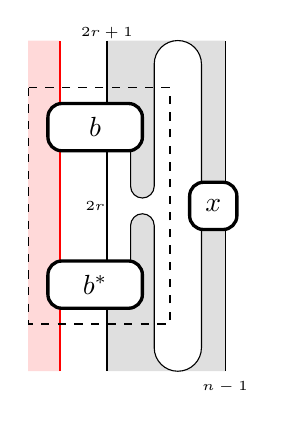
\begin{tikzpicture}[baseline]
	\fill[ctwoshading] (-1,-2.1) -- (-1,2.1) -- (-.6,2.1) -- (-.6,-2.1) -- (-1,-2.1);
	\fill[shaded] (0,2.1) -- (0,0.7) -- (0.3,0.7) -- (0.3,0.25)arc (-180:0:.15cm)-- (0.6,1.8)arc(180:0:.3cm) -- (1.2,-1.8) arc(0:-180:0.3cm) -- (0.6,-0.25) arc(0:180:0.15cm) -- (0.3,-0.7) -- (0,-.7) -- (0,-2.1) -- (1.5,-2.1) -- (1.5,2.1);
	\draw[thick,red] (-0.6,-2.1) -- (-0.6,2.1);
	\draw (0.3,.7)--(0.3,0.25) arc (-180:0:.15cm)-- (0.6,1.8) arc(180:0:.3cm) -- (1.2,.15);
	\draw (0.3,-.7)--(0.3,-0.25) arc (180:0:.15cm)-- (0.6,-1.8) arc(-180:0:.3cm) -- (1.2,-.15);
	\draw (0,-2.1) -- (0,2.1);
	\draw (1.5,-2.1) -- (1.5,2.1);
	\draw[dashed] (-1,1.5) --  (-1,-1.5) --  (0.8,-1.5) --  (0.8,1.5) -- (-1,1.5);
	\roundNbox{unshaded}{(1.35,0)}{.3}{0}{0}{$x$}
	\roundNbox{unshaded}{(0.15,1)}{.3}{0.6}{0}{$b$}
	\roundNbox{unshaded}{(0.15,-1)}{.3}{0.6}{0}{$b^\ast$}
	\node at (1.5,-2.3) {\tiny{$n-1$}};
	\node at (0,2.2) {\tiny{$2r+1$}};
	\node at (-.15,0) {\tiny{$2r$}};
\end{tikzpicture} 
=
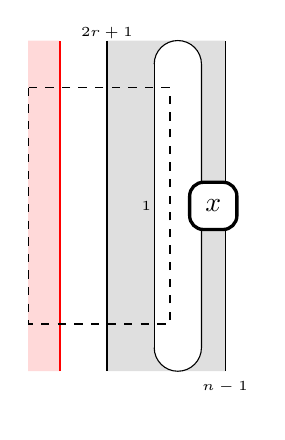
\begin{tikzpicture}[baseline]
	\fill[ctwoshading] (-1,-2.1) -- (-1,2.1) -- (-.6,2.1) -- (-.6,-2.1) -- (-1,-2.1);
	\fill[shaded] (0,2.1) -- (1.5,2.1) -- (1.5,-2.1) -- (0,-2.1) -- (0,2.1);
	\fill[unshaded] (0.6,1.8) arc(180:0:.3cm) -- (1.2,-1.8)arc(0:-180:0.3cm) -- (0.6,1.8); 
	\draw[thick,red] (-0.6,-2.1) -- (-0.6,2.1);
	\draw (0.6,1.8) arc(180:0:.3cm) -- (1.2,.15);
	\draw (0.6,-1.8) arc(-180:0:.3cm) -- (1.2,-.15);
	\draw (0.6,1.8) -- (0.6,-1.8);
	\draw (0,-2.1) -- (0,2.1);
	\draw (1.5,-2.1) -- (1.5,2.1);
	\draw[dashed] (-1,1.5) --  (-1,-1.5) --  (0.8,-1.5) --  (0.8,1.5) -- (-1,1.5);
	\roundNbox{unshaded}{(1.35,0)}{.3}{0}{0}{$x$}
	\node at (1.5,-2.3) {\tiny{$n-1$}};
	\node at (0,2.2) {\tiny{$2r+1$}};
	\node at (0.5,0) {\tiny{$1$}};
\end{tikzpicture} 
=
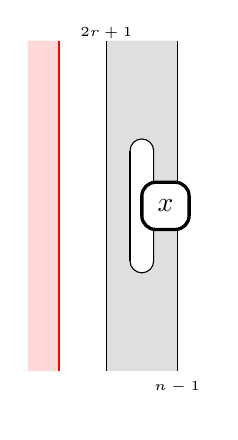
\begin{tikzpicture}[baseline]
	\fill[ctwoshading] (-1,-2.1) -- (-1,2.1) -- (-.6,2.1) -- (-.6,-2.1) -- (-1,-2.1);
	\fill[shaded] (0,2.1) -- (.9,2.1) -- (.9,-2.1) -- (0,-2.1) -- (0,2.1);
	\fill[unshaded] (0.3,0.7) arc(180:0:.15cm) -- (0.6,-0.7)arc(0:-180:0.15cm) -- (0.3,0.7); 
	\draw[thick,red] (-0.6,-2.1) -- (-0.6,2.1);
	\draw (0.3,0.7) arc(180:0:.15cm) -- (0.6,.15);
	\draw (0.3,-0.7) arc(-180:0:.15cm) -- (0.6,-.15);
	\draw (0.3,0.7) -- (0.3,-0.7);
	\draw (0,-2.1) -- (0,2.1);
	\draw (0.9,-2.1) -- (0.9,2.1);
	\roundNbox{unshaded}{(0.75,0)}{.3}{0}{0}{$x$}
	\node at (0.9,-2.3) {\tiny{$n-1$}};
	\node at (0,2.2) {\tiny{$2r+1$}};
\end{tikzpicture}
	\]
  \end{minipage}
}
Clearly, the last diagram depicts an element of  $\Phi(Q_{\bullet})$. In fact, we have $\gamma^+_n(\Phi(x)) =\Phi(\gamma^+_n(x))$.
\end{enumerate}
\item The negative inclusion $i^{-}_{n} : P_{n,-} \to P_{n+1,+}$ is just the identity on the relative commutant planar algebra. Let $\overline{i^{-}_{n}}$ be the negative inclusion in $Q_{n,\pm}$. Graphically, this is equivalent to adding a string on the left. Thus, for $x$ in $Q_{n,-}$ we have that:
\[
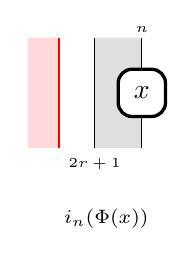
\begin{tikzpicture}[baseline]
	\fill[ctwoshading] (-.9,-.7) -- (-0.9,.7) -- (-1.3,0.7) -- (-1.3,-0.7) -- (-0.9,-0.7);
	\fill[shaded] (-0.45,-0.7) -- (-0.45,0.7) -- (0.15,0.7) -- (0.15,-0.7) -- (-0.45,-0.7);
	\draw[red, thick] (-0.9,-0.7) -- (-0.9,0.7);
	\draw (-0.45,-0.7) -- (-0.45,0.7);
	\draw (0.15,-0.7) -- (0.15,0.7);
	\roundNbox{unshaded}{(0.15,0)}{.3}{0}{0}{$x$};
	\node at (0.15,0.8){\tiny{$n$}};
	\node at (-0.45, -0.9){\tiny{$2r+1$}};
	\node at (-0.30,-1.6){\scriptsize{$i_n(\Phi(x))$}};
\end{tikzpicture}
\quad
=
\quad
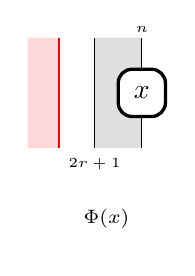
\begin{tikzpicture}[baseline]
	\fill[ctwoshading] (-.9,-.7) -- (-0.9,.7) -- (-1.3,0.7) -- (-1.3,-0.7) -- (-0.9,-0.7);
	\fill[shaded] (-0.45,-0.7) -- (-0.45,0.7) -- (0.15,0.7) -- (0.15,-0.7) -- (-0.45,-0.7);
	\draw[red, thick] (-0.9,-0.7) -- (-0.9,0.7);
	\draw (-0.45,-0.7) -- (-0.45,0.7);
	\draw (0.15,-0.7) -- (0.15,0.7);
	\roundNbox{unshaded}{(0.15,0)}{.3}{0}{0}{$x$};
	\node at (0.15,0.8){\tiny{$n$}};
	\node at (-0.45, -0.9){\tiny{$2r+1$}};
	\node at (-0.30,-1.6){\scriptsize{$\Phi(x)$}};
\end{tikzpicture}
\quad
=
\quad
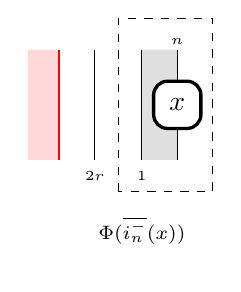
\begin{tikzpicture}[baseline]
	\fill[ctwoshading] (-.9,-.7) -- (-0.9,.7) -- (-1.3,0.7) -- (-1.3,-0.7) -- (-0.9,-0.7);
	\fill[shaded] (0.15,-0.7) -- (0.15,0.7) -- (0.6,0.7) -- (0.6,-0.7) -- (0.15,-0.7);
	\draw[red, thick] (-0.9,-0.7) -- (-0.9,0.7);
	\draw (-0.45,-0.7) -- (-0.45,0.7);
	\draw (0.6,-0.7) -- (0.6,0.7);
	\draw (0.15,-0.7) -- (0.15,0.7);
	\roundNbox{unshaded}{(.6,0)}{0.3}{0}{0}{$x$};
	\draw[dashed] (-0.15,-1.1) -- (-0.15,1.1) -- (1.05,1.1) --  (1.05,-1.1) -- (-0.15,-1.1);
	\node at (0.6,0.8){\tiny{$n$}};
	\node at (-0.45, -0.9){\tiny{$2r$}};
	\node at (0.15,-0.9){\tiny{1}};
	\node at (0.15,-1.6){\scriptsize{$\Phi(\overline{i^{-}_{n}}(x))$}};
\end{tikzpicture}\]
\end{enumerate}
\end{proof}

We have checked that $\Phi(Q_{\bullet}) \subset P_{\bullet}$ is a planar $\ast$-algebra inclusion. Let $G_\bullet$ be the bipartite graph planar algebra of the fusion graph of $x$ acting on $\cM$. Then by Theorem 3.33 in \cite{penneys}, 
we know that $P_\bullet$ is a planar $\ast$-algebra isomorphic to $G_\bullet$. Thus, we have an embedding $Q_\bullet$ into $G_\bullet$.

\begin{cor}[The Embedding Theorem]
	A subfactor planar algebra $Q_\bullet$ can be embedded into the bipartite graph planar algebra of the fusion graph of a cyclic $Q_\bullet$-module.
\end{cor}

In particular, by considering $(Q_\bullet,1)$ as a cyclic right module over itself, we recover the main result of \cite{penneys} as a corollary, and by instead considering $Q_\bullet$ as a left module, we obtain an embedding into the graph planar algebra of the dual principle graph: 

\begin{cor}
Let $Q_{\bullet}$ be a finite depth subfactor planar algebra then there is an embedding of $Q_{\bullet}$ into the bipartite graph planar algebra of the principal graph of $Q_{\bullet}$, and the bipartite graph planar algebra of the dual principal graph of $Q_{\bullet}$.
\end{cor}

%%%%%%%%%%%%%%%%%%%%%%%%%%%%%%%%%%%%%%%%%%%%%%%%%%%%%%%
\subsection{Invariance of the embedding}
As the observant reader may noted, for any $m\in \cM$ one may obtain a different embedding of the subfactor planar algebra $Q_\bullet$ into $G_{\bullet}$ the bipartite graph planar algebra for the fusion graph given by tensoring with the strand, $x$. We will show that differ only by automorphisms of $G_{\bullet}$. Notice that show this it suffices to show that if $\R_{\bullet}$ and $S_{\bullet}$ are canonical planar algebras constructed through the process in section 4, and $\phi$ and $\phi'$ are the respective embeddings of $Q_{\bullet}$ into each then there is some isomorphism $\Psi:R_{\bullet}\rightarrow R{\bullet}$ such that the following triangle commutes:

$$
  \begin{tikzcd}
    Q_{\bullet} \arrow{r}{\phi} \arrow[swap]{dr}{\phi'} & R_{\bullet} \arrow{d}{\Psi} \\
     & S_{\bullet}
  \end{tikzcd}
$$  
It suffices to show this because by \ref{planaralgebraisomorphism} we have that $R_{\bullet}$ and $S_{\bullet}$ are both isomorphic to $G_{\bullet}$ so $\phi$ lifts to an automorphism of $G_{\bullet}$. First we will show this for the special where we take two different values for $r$ such that the inclusion $A_{2r}\subseteq A_{2r+1}\subseteq A_{2r+2}$ is standard. The following lemma is a direct consequence of the shift isomorphism discussed in section \ref{example}.

\begin{prop}
Let $R_{\bullet}$ and $S_{\bullet}$ be the canonical planar algebras given by the inclusions $A_{2r}\subseteq A_{2r+1}$ and $A_{2s}\subseteq A_{2s+1}$ where $A_n:=\End_{\widetilde{\cC}}(m\otimes \xalt)$ for some $m\in \cC_{20}$. Let $\phi$ and $\phi'$ be the embeddings of $Q_{\bullet}$ into $R_{\bullet}$ and $S_{\bullet}$ respectively. Then thereis some isomorphism $\Psi:R_{\bullet}\rightarrow R_{\bullet}$ such that the following triangle commutes:

$$
  \begin{tikzcd}
    Q_{\bullet} \arrow{r}{\phi} \arrow[swap]{dr}{\phi'} & R_{\bullet} \arrow{d}{\Psi} \\
     & S_{\bullet}
  \end{tikzcd}
$$  
\end{prop}




\bibliographystyle{amsalpha}
{\footnotesize{
\bibliography{embedding_theorem}
}}
\end{document}
